\documentclass[a4paper]{article}

% Use the postscript times font!
\usepackage{times}
\usepackage{soul}
\usepackage[hyphens]{url}
\usepackage[hidelinks]{hyperref}
\usepackage[utf8]{inputenc}
\usepackage[small]{caption}
\usepackage{amsmath}
\usepackage{amsfonts}
\usepackage{graphicx}
\usepackage{subcaption}
\usepackage{amsmath,amssymb}
\usepackage{booktabs}
\usepackage[a4paper, portrait, margin=1in]{geometry}
\urlstyle{same}

\usepackage{parskip}

% the following package is optional:
%\usepackage{latexsym} 

\title{
\includegraphics[scale=0.75]{images/unblogo.jpg}\\CS6735 Programming Project Report}

\makeatletter
\renewcommand\@date{{%
  \vspace{-\baselineskip}%
  \large\centering
  \begin{tabular}{@{}c@{}}
    Ethan Garnier\textsuperscript{1} \\
    \normalsize ethan.garnier78@unb.ca 
  \end{tabular}%
  \hspace{3mm}
  \begin{tabular}{@{}c@{}}
    Matthew Tidd\textsuperscript{2} \\
    \normalsize mtidd2@unb.ca
  \end{tabular}
  \hspace{3mm}
  \begin{tabular}{@{}c@{}}
    Minh Nguyen\textsuperscript{2} \\
    \normalsize mnguyen6@unb.ca
  \end{tabular}
  
  \bigskip

  \textsuperscript{1}Department of Electrical and Computer Engineering, UNB\par
  \textsuperscript{2}Department of Mechanical Engineering, UNB

  \bigskip

  \today
}}
\makeatother

\begin{document}

\maketitle

\begin{abstract}
    In the field of Artificial Intelligence and Machine Learning, it can be very easy for the complexities of learning models to be obscured away behind the black boxes that are machine learning libraries. Despite the ease of use by which these libraries present, they do not always provide a complete understanding of how the learning is taking place. To truly grasp and take advantage of machine learning, one must understand the inner workings of the learning models being applied. This assignment saw students manually implement three machine learning models to truly test their understanding of these models and how they function. These models were: Adaboost with an ID3 weak base learner, an Artificial Neural Network with back-propagation, and Naïve Bayes. In addition to manually implementing these three learning models from scratch, two machine learning problems were solved using pre-existing machine learning libraries. These problems included developing a Deep Fully-Connected Feed-Forward Artificial Neural Network, and a Convolutional Neural Network to be trained and tested on the MNIST dataset of handwritten digits.
\end{abstract}

\newpage

\section{Introduction}

\section{Adaboost with ID3 Base Learner}
The Adaptive Boosting (Adaboost) classification algorithm was successfully implemented using the Python 3 programming language. The version of Adaboost implemented used the Iterative Dichotomiser 3 (ID3) decision tree learning algorithm as a weak learner. This algorithm was trained on a dataset of English alphabet character image features and used to identify letters of the alphabet based on these features, i.e., letter recognition.

\subsection{Adaboost}
Adaboost is a boosted classifier that uses multiple weak hypotheses to build a single, strong hypothesis to be used for classification. These weak hypotheses are initially learned through a weak base learner algorithm, with the performance of these weak hypotheses dictating their weight in the final, strong hypothesis. To accomplish this, Adaboost first assigns an initial weight of $1/N$ to every training example, where $N$ is the number of training examples. Upon training of a weak hypothesis, Adaboost sums the weight of all misclassified examples against the trained weak hypothesis.  This sum, called the $error$ or $\epsilon$, is used to calculate the weight, or $\alpha$, for the given weak hypothesis according to Equation~\ref{eq:weak-h-alpha}.

\begin{equation}
    \label{eq:weak-h-alpha}
    \alpha = \frac{1}{2}\ln\left(\frac{1-\epsilon}{\epsilon}\right)
\end{equation}

This process of training weak learners and calculating the $\alpha$ of those weak learners is repeated $T$ times. On each iteration of the boosting algorithm, $t \le T$, the weights of all $N$ training examples for the next iteration, $w_{i, t+1}$, are updated according to Equation~\ref{eq:example-weight-update}.

\begin{equation}
    \label{eq:example-weight-update}
    w_{i, t+1} =
    \begin{cases} 
      w_{i,t}e^{-\alpha_t} & h_t(x_i) = y_i \\
      w_{i,t}e^{\alpha_t} & h_t(x_i) \ne y_i \\
   \end{cases}
\end{equation}

Where $w_{i,t}$ is the weight of training example $i$ for the current iteration, $\alpha_t$ is the weight of the most recently learned weak hypothesis, $h_t(x_i)$ is the classification of training example $i$ using this weak hypothesis, and $y_i$ is the correct classification of example $i$. These newly calculated weights are then normalized to ensure the sum of all training example weights is one. As can be seen from Equation~\ref{eq:example-weight-update}, the weight of incorrectly classified training examples is increased, whereas correctly classified examples have their weights decreased. The reason for this is that Adaboost wants the weak base learners to place extra emphasis on learning the incorrectly classified examples to produce a more accurate result in the end. Details on how this is executed lies within the chosen weak base learner algorithm. 

\subsection{ID3}
For this implementation of Adaboost, the ID3 algorithm was chosen as the weak base learner. ID3 is a greedy, recursive learning algorithm that generates binary decision trees from a given dataset, \textit{S}, where each internal node represents a feature by which \textit{S} is split, and leaf nodes represent a classification for the remaining examples in \textit{S}. The inductive bias of the ID3 algorithm is that it prefers shorter decision trees, building off the idea that a short hypothesis that fits the data well is unlikely to be a coincidence, as opposed to a larger hypothesis. This bias of the ID3 algorithm is enforced through its statistically based splitting criteria. At each internal node, the entropy of the dataset \textit{S} is calculated based on Equation~\ref{eq:entropy}.

\begin{equation}
    \label{eq:entropy}
    Entropy(S) = -\sum_{x \in X} p(x)log(p(x))
\end{equation}

Where $X$ is the set of all classifications in $S$, and $p(x)$ is the probability of a given classification in $S$. Once the entropy for $S$ is calculated, every attribute value for every attribute in $S$ is examined as a potential split attribute value. This is done by calculating the information gain of splitting $S$ based on that attribute value according to Equation~\ref{eq:info-gain}.

\begin{equation}
    \label{eq:info-gain}
    Gain(S, A, V) = Entropy(S) - \left(\frac{|S_{\le V}|}{|S|}\times Entropy(S_{\le V}) + \frac{|S_{> V}|}{|S|}\times Entropy(S_{> V}) \right)
\end{equation}

Where $S_{\le V}$ is the subset of training examples in $S$ whose value for attribute $A$ is less than or equal to $V$, and $S_{> V}$ is the subset of training examples in $S$ whose value for attribute $A$ is greater than $V$. The largest information gain calculated for the current internal node determines the feature and feature value by which the data will be split going to the next level of the decision tree. The fact that there are only two splits for each internal node shows that this is a binary decision tree. This splitting of training examples and building of binary decision tree continues until one of the given three base cases are met:
\begin{enumerate}
    \item Base Case 1 - Every training example in \textit{S} belong to the same class. If this is the case, then return that class.

    \item Base Case 2 - There are no remaining attributes to split the data off of. If this is the case, then return the class of majority for the training examples in \textit{S}.

    \item Base Case 3 - There are no training examples in \textit{S}. If this is the case, then return the class of majority for the training examples of the parent node.
\end{enumerate}
Base case 3 is especially important, as it is this which provides the ID3 algorithm with its generalizing power. A slight change to the ID3 algorithm was made in this implementation to account for it being used as a weak base learner in Adaboost. As previously mentioned, Adaboost will update the weights of each training example over its iterations to favor the incorrectly classified examples. The weak base learner, ID3 in this case, must therefore take these weights into account to try extra hard to correctly learn these incorrectly classified examples. This was accomplished by modifying Equation~\ref{eq:info-gain} to account for the total weight of the example subsets. This can be seen in Equation~\ref{eq:weighted-info-gain}.

\begin{equation}
    \label{eq:weighted-info-gain}
    Gain(S, A, V) = Entropy(S) - \left(\frac{\sum_{e \in S_{\le V}}w_e}{|S|}\times Entropy(S_{\le V}) + \frac{\sum_{e \in S_{> V}}w_e}{|S|}\times Entropy(S_{> V}) \right)
\end{equation}

\subsection{Predicting with Adaboost}
Once the $T$ weak hypotheses have been trained and each has their own associated weight $\alpha_t$, it is time to begin classifying test data. For each testing example $x_i$, $T$ classifications are acquired by classifying that example with each of the trained weak hypothesis. For each unique classification of $x_i$, the weights, or $\alpha_t$, of all base hypotheses that gave that classification are summed and this sum represents the weight of this classification for $x_i$. The classification with the largest weight becomes the final, or returned classification for testing example $x_i$. This process is repeated for all testing examples.

\subsection{Implementation Details}
This section will outline all details related to this implementation of Adaboost and the ID3 algorithm.

\subsubsection{Development Platform and Libraries}
As was previously mentioned, all code written to implement the Adaboost and ID3 algorithms was written in Python 3. This code was written to run on a Windows operation system, but will run on any system that can run the Python programming language. All development was conducted through the Visual Studios Code text editor, and code versioning was controlled through Git to a remote repository hosted on GitHub. The Adaboost and ID3 algorithms were written completely from scratch using only Python's built-in functions, the \textit{Numpy} Python library for mathematical operations, and the \textit{Pandas} Python library for data manipulation and representation. The \textit{scikit-learn} maching learning Python library was used for pre-processing of training and testing data, as well as for evaluating the performance of the manually implemented algorithms. This machine learning library was not included or used in any of the Adaboost or ID3 algorithm implementations. The \textit{matplotlib} and \textit{seaborn} Python libraries were used to provide statistical data visualizations for the algorithm's results.

\subsubsection{Program Structure}
Python classes were used to structure the various components of this Adaboost implementation. These classes included: \textit{AdaBoost} (adaboost.py), \textit{ID3Classifier} (id3.py), and \textit{BinaryDecisionTree} (tree.py). By following an object oriented approach, different instances of the learning algorithms could be instantiated with different hyper-parameters and then re-used when needed. This, in addition to allowing these classes to keep track of their own internal state while training, significantly cleaned up and optimized the code. For example, the \textit{AdaBoost} class has it's own internal member variables named \textit{models} and \textit{alphas} which store the trained weak hypotheses and their corresponding weights, respectively. This means that once the \textit{AdaBoost} models have been trained, these models and their weights can easily be accessed through these member variables, vastly reducing the amount of code required to keep track of this state. In addition to this, the \textit{ID3Classifier} class contains two private static methods used to calculate the entropy and information gain throughout its training process.

\subsubsection{Data-Structures}
The Dataframe data structure, as part of the \textit{Pandas} library, is a data structure that allows for data to be represented in a two-dimensional tabular format and was used extensively throughout this project. Using Dataframes allowed for the training and testing data to easily be extracted, segmented, manipulated, and represented throughout the entire training and classification process. Although operations on Dataframes are extremely slow, they also allow for the data to be exported to a two-dimensional Numpy array, and this feature was used a lot for data manipulation and calculations. Finally, Dataframes were leveraged to store training and classification results of the Adaboost algorithm in a tabular format and to export these results to a .csv file.

A binary tree data structure was manually implemented in Python to fulfill the decision tree output of the ID3 algorithm. This binary tree implementation, named \textit{BinaryDecisionTree} in tree.py, is a recursive tree data structure that possesses four attributes: 1) a split feature index, 2) a split feature value, 3) a truth branch, 4) a false branch. The split feature index of the \textit{BinaryDecisionTree} is an integer value that represents the feature this node splits on in the training data. Instead of storing the name of the feature as a string, the index of the feature in the list of feature names is stored. This is done to improve performance. The split feature value is exactly as the name describes, it is the value of the split feature by which this node splits the data on. The truth branch is a reference to another \textit{BinaryDecisionTree} object, hence the recursive nature of the data structure. When traversing the \textit{BinaryDecisionTree}, this branch is evaluated when a provided feature value is greater than the split feature value of this node. Finally, the false branch is a reference to another \textit{BinaryDecisionTree} object that is evaluated when a provided feature value is less than or equal to the split feature value of this node. The form of the trees built by the \textit{BinaryDecisionTree} object can be seen in Figure~\ref{fig:binary-decision-tree}. 

\begin{figure}[h]
    \centering
    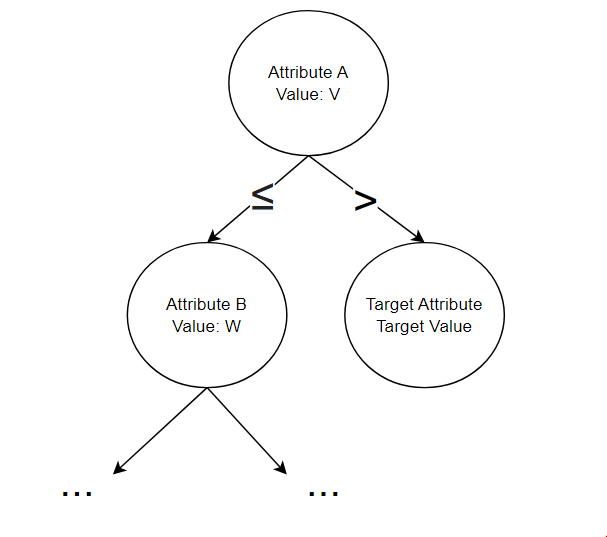
\includegraphics[scale=0.55]{images/binary-decision-tree.PNG}
    \caption{Binary decision tree created by \textit{BinaryDecisionTree} class.}
    \label{fig:binary-decision-tree}
\end{figure}

As can be seen in Figure~\ref{fig:binary-decision-tree}, leaf nodes of the tree generated by \textit{BinaryDecisionTree} have their split feature set to the target attribute of the data set, and the split feature value is the classification of the target attribute. The true and false branches are empty. As such, predictions can be made on a learned \textit{BinaryDecisionTree} for a given testing example by simply following the trees branches, checking the testing example's feature values with the split feature values at each node, until a leaf is reached where the classification for the testing example is returned.

\subsubsection{Algorithm Hyper-Parameters}
Two hyper-parameters were implemented for this Adaboost with ID3 base learner implementation. These hyper-parameters include: 1) the maximum tree depth of the learned binary decision trees, and 2) the number of weak hypotheses learned by Adaboost. 

The maximum tree depth of the learned binary decision tree is a hyper-parameter of the ID3 algorithm implementation, and it sets a limit on the maximum depth of recursion of the algorithm. This depth was monitored as a \textit{depth} parameter incremented on each recursive call. When the maximum depth was reached, the target value of majority in the current data set was returned as the leaf node. If the caller did not specify a maximum tree depth, then a tree depth of infinity was set, which essentially means the algorithm would only return a leaf node if one of its original three base cases were hit. It was experimentally determined, as can be seen in Figure~\ref{fig:depth-hyper-param}, that placing a limit on the depth of the trained binary decision tree less than the number of features in the data set actually reduces classification accuracy. For context, Figure~\ref{fig:depth-hyper-param} used a dataset with 16 features. This makes intuitive sense, as each node splits on a single feature, so there can only ever be a tree as deep as the number of features. Also, if we force a tree to terminate early, then we are forcing it to over generalize the data. Either way, this hyper-parameter remained as reducing the depth of the tree significantly improves training and classification performance. 

\begin{figure}[h]
    \centering
    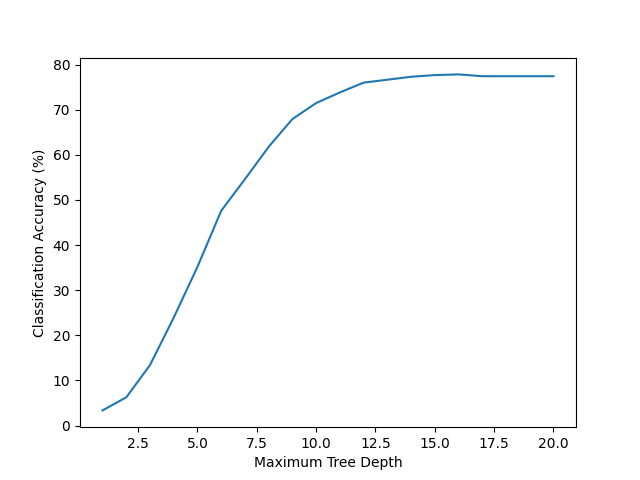
\includegraphics[scale=0.7]{images/tree-depth-plot.png}
    \caption{Accuracy of classification vs. maximum tree depth of learned binary decision tree by ID3 algorithm.}
    \label{fig:depth-hyper-param}
\end{figure}

The second hyper-parameter implemented, the number of weak hypotheses learned by the Adaboost algorithm, is a hyper-parameter of the Adaboost algorithm that controls the number of models trained by the weak base learner for a single Adaboost training session. This hyper-parameter has direct influence on the performance of the Adaboost algorithm, both from a time point-of-view and an accuracy point-of-view. The more weak hypotheses trained, the longer training will take; however, the more accurate classification can become. It was experimentally determined that 14 is the optimal number of weak hypotheses to learn as it maximizes the classification accuracy while keeping the training time as low as possible. Figure~\ref{fig:estimator-hyper-param} demonstrates how at 14 weak hypotheses, the classification accuracy of the Adaboost algorithm reaches an asymptote. Although this is only for a particular split of the dataset, it remains consistent. Figure~\ref{fig:estimator-time} shows how the time taken for training the Adaboost algorithm increases linearly with the number of weak hypotheses learned by the algorithm. As such, it is optimal to use 14 weak hypotheses to maximize classification accuracy while ensuring training time doesn't continue to increase.

\begin{figure}[h]
    \centering
    \begin{subfigure}[t]{0.48\textwidth}
        \centering
        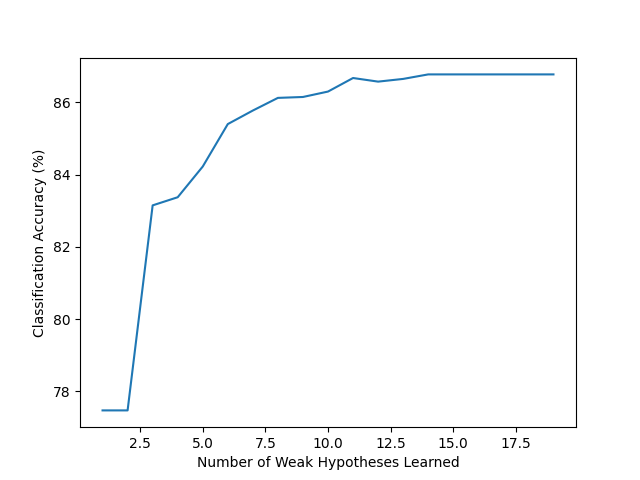
\includegraphics[width=\linewidth]{images/n-weak-hypotheses-plot.png}
        \caption{}
        \label{fig:estimator-hyper-param}
    \end{subfigure}%
    ~ 
    \begin{subfigure}[t]{0.48\textwidth}
        \centering
        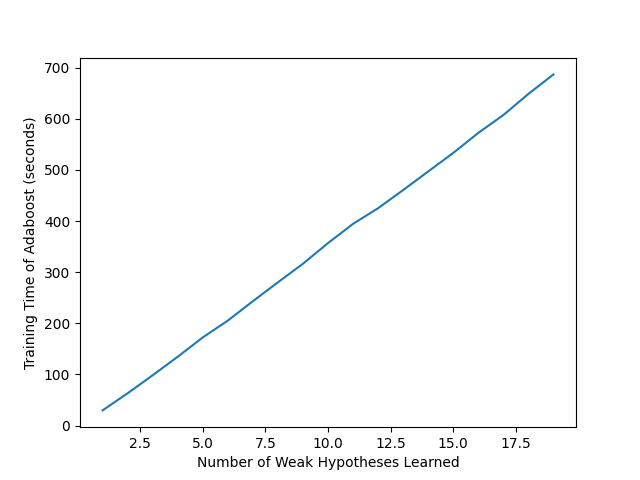
\includegraphics[width=\linewidth]{images/adaboost-training-time.png}
        \caption{}
        \label{fig:estimator-time}
    \end{subfigure}

    \caption{Performance of the number of weak hypotheses trained by Adaboost algorithm during training vs. (a) classification accuracy, and (b) time taken to train the model.}
    \label{fig:adaboost-hyper-param}
\end{figure}   

\subsection{Dataset Details}
This section will outline all details related to dataset used to train and test the Adaboost implementation. 

\subsubsection{Description of Dataset}
The dataset was taken from the UC Irvine Machine Learning Repository and has the ID 59 within this repository. The goal of the dataset is to identify each entry as a capital letter from the English alphabet based on 16 primitive numerical attributes extracted from a black-and-white image of the letter that the entry represents. The dataset contains 20 thousand entries with 17 columns for each entry, 16 columns being the previously mentioned primitive numerical attributes, and the final column being the classification of the entry, a letter in this case. These 16 primitive numerical attributes, or features in the context of machine learning, are integer values between 0 and 15 and are described as the following:
\begin{enumerate}
    \item x-box - Horizontal position of box.
    \item y-box - Vertical position of box.
    \item width - Width of box.
    \item hight - Height of box.
    \item onpix - Total number on pixels.
    \item x-bar - Mean x of on pixels in box.
    \item y-bar - Mean y of on pixels in box.
    \item x2bar - Mean x variance.
    \item y2bar - Mean y variance.
    \item xybar - Mean x y correlation.
    \item x2ybr - Mean of x * x * y.
    \item xy2br - Mean of x * y * y.
    \item x-ege - Mean edge count left to right.
    \item xegvy - Correlation of x-ege with y.
    \item y-ege - Mean edge count bottom to top.
    \item yegvx - Correlation of y-ege with x.
\end{enumerate}

The total number of classes in this dataset is 26, representing the number of capital letters in the English alphabet. The distribution of classes within the dataset is nearly uniform, as can be seen in Figure~\ref{fig:class-histogram}. As such, no re-sampling of data was needed.

\begin{figure}[h]
    \centering
    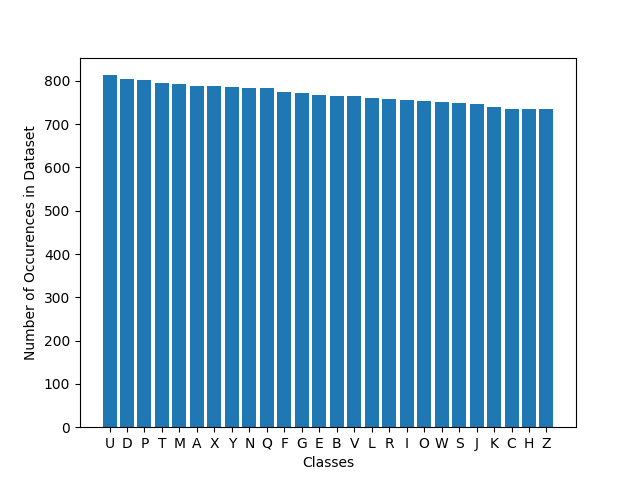
\includegraphics[scale=0.7]{images/class-distribution.png}
    \caption{Distribution of classes within the Letter Distribution dataset.}
    \label{fig:class-histogram}
\end{figure}

\subsubsection{Pre-Processing}
As previously mentioned, there are no missing values within the dataset used. As such, no pre-processing of the data to remove partial entries was required. The only pre-processing performed on the dataset was to split the data into testing and training datasets using the \textit{train\_test\_split()} function from the \textit{scikit-learn} machine learning library. A split of 80\%/20\% (16000/4000) was used for training and testing, respectively, as this was the split suggested by UC Irvine on the dataset's webpage. As such, in all results presented in the next sections, the Adaboost algorithm was trained on 16 000 randomly selected entries, and tested on the remaining 4000 entries of the dataset.

\subsection{Experimental Results}
The above discussed Adaboost algorithm with ID3 as a weak base learner implementation was tested extensively and the results of this testing can be seen in Table~\ref{tbl:adaboost-results}. As previously mentioned, these results were achieved by training the algorithm on 16 000 randomly sampled entries of the dataset, and tested on the remaining 4000 entries of the dataset. The seeds, or \textit{random\_states}, of the sampling is also reported in the table for reproducibility. The hyper-parameters were set to their previously mentioned optimal values of 16 for the maximum depth of a learned binary decision tree, and 14 for the number of weak hypotheses learned by the Adaboost algorithm.

\begin{table}[h!]
    \centering
    \begin{tabular}{||c c c c c||} 
        \hline
        Test \# & Seed & Accuracy (\%)  & Training Time (s) & Classification Time (s) \\ [0.5ex] 
        \hline\hline
        1 & 500864380 & 85.33 & 509.20 & 0.0897 \\
        \hline
        2 & 434317629 & 85.45 & 498.24 & 0.0888 \\
        \hline
        3 & 81483430 & 84.40 & 489.30 & 0.0897 \\
        \hline
        4 & 794073002 & 86.28 & 492.81 & 0.0891 \\
        \hline
        5 & 278379451 & 84.10 & 492.79 & 0.0898 \\
        \hline
        6 & 1019885152 & 84.65 & 483.37 & 0.0877 \\
        \hline
        7 & 880373647 & 85.93 & 486.33 & 0.0875 \\
        \hline
        8 & 244411609 & 85.88 & 487.19 & 0.0906 \\
        \hline
        9 & 573119018 & 83.80 & 485.92 & 0.0893 \\ 
        \hline
        10 & 496202245 & 83.03 & 487.38 & 0.0896 \\
        \hline
        11 & 136944384 & 84.18 & 500.03 & 0.0905 \\
        \hline
        12 & 131276866 & 85.80 & 486.27 & 0.0868 \\
        \hline
        13 & 276617434 & 86.70 & 482.18 & 0.0886 \\
        \hline
        14 & 817708150 & 86.60 & 478.75 & 0.0892 \\
        \hline
        15 & 44078284 & 86.68 & 505.69 & 0.0908 \\ [1ex]
        \hline
    \end{tabular}
    \caption{Results of training Adaboost implementation on 16 000 randomly sampled examples and classifying the remaining 4000 examples with maximum tree depth of 16 and 14 weak base hypotheses learned.}
    \label{tbl:adaboost-results}
\end{table}

The mean classification accuracy of the results presented in Table~\ref{tbl:adaboost-results} is 85.254\%, with the mean training and classification times being 491.03 seconds and 0.08918 seconds, respectively. Despite not achieving 100\% accuracy, the Adaboost implementation is still a success in our opinion as it is a completely from scratch implementation. The lack of accuracy in classification may come from the weighted feature info gain calculation being employed, referenced in Equation~\ref{eq:weighted-info-gain}, to place more emphasis on previously incorrectly classified examples. As for the training time, ID3 is a greedy algorithm, as such it is expected to have a longer execution time. Much work was done in the ID3 implementation to ensure all math operations were vectorized within the Python programming language to minimize the amount of looping and memory copies required. No parallelization was employed as to not over complicate the implementation, yet the routine for determining the split feature can easily be parallelized as determining the split feature based on weighted info gain can be done independently of other features.

The confusion matrix of the test with the highest accuracy, test 13 with seed 276617434, can be seen in Figure~\ref{fig:confusion-matrix}. The confusion matrix helps highlight the number of examples that were incorrectly classified, and what those incorrect classifications were compared to the correct classifications. As such, a strong diagonal of the matrix indicates high classification accuracy, as can be seen in Figure~\ref{fig:confusion-matrix}.

\begin{figure}[h!]
    \centering
    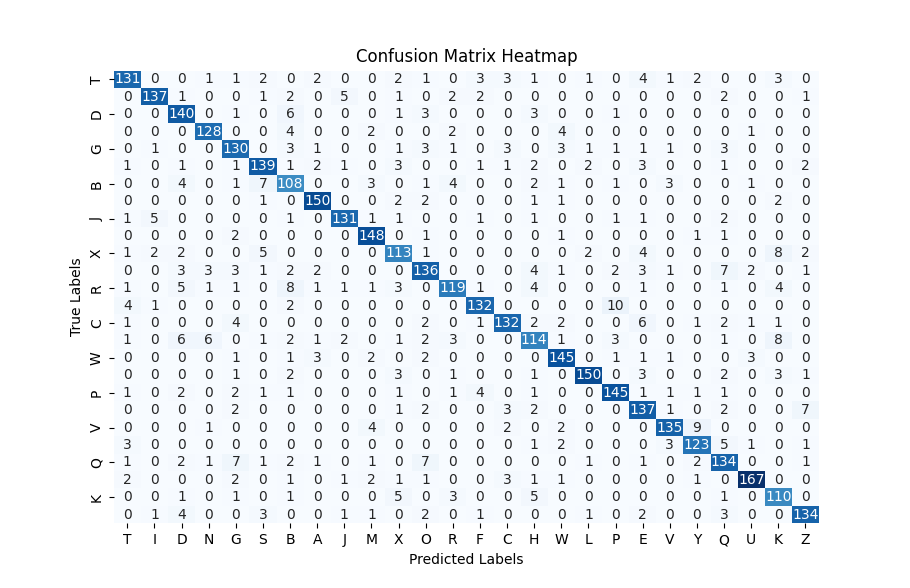
\includegraphics[scale=0.65]{images/confusion-matrix.png}
    \caption{Confusion matrix of training/classification results with seed 276617434.}
    \label{fig:confusion-matrix}
\end{figure}


\newpage

\section{ANN with Backpropagation}

An Artificial Neural Network with backpropagation was successfully implemented using the Python 3 programming language. The artificial neural network that was created featured a simplistic design, utilizing only one hidden layer while simultaneously yielding great results. This algorithm was trained on a dataset that consisted of features computed from digitized images of fine needle aspirate of breast mass, describing charactersitics of the cell nuclei present in the image. The objective was classification of cell mass as either benign or malignant.

\subsection{Artificial Neural Networks}

As mentioned, this section of the programming project saw the implementation of an artificial neural network from scratch. Artificial neural networks, or neural networks, are a machine learning technique that seek to mimic the biological neural networks found within human brains. A neural network consists of connected ``units", or nodes, that are called neurons. These neurons are designed such that they mimic the neurons found within a human brain, in the sense that they will not ``fire'', so to speak, if the input signal is not larger than a certain threshold. This thresholding is achieved through the use of an activation function, which ensures that important features that are interesting enough to be learned are actually learned by the network as they exceed the threshold. The output of a given neuron is therefore calculated by applying the activation function to the weighted sum of the inputs to that neuron. Neural networks are composed of three distinct layers, those being the input layer, the hidden layer, and the output layer. The input signal is first sent through the input layer, which takes in the data and sends it to the subsequent layers, known as the hidden layers. The hidden layers serve as an intermediary layer between the first layer and the last layer, the output layer. It is within these hidden layers that the input becomes further and further abstracted, and a new representation is learned that extracts the hidden relationship between the input features. 


For this assignment, as mentioned, a neural network was created with three layers: one input, one hidden, and one output. Justification for the choice of this structure can be found within Section \ref{ANNhyperparameterselection}. As such, the general structure of the neural network implemented is given by Figure \ref{fig:annstructure}:

\begin{figure}[h]
    \centering
    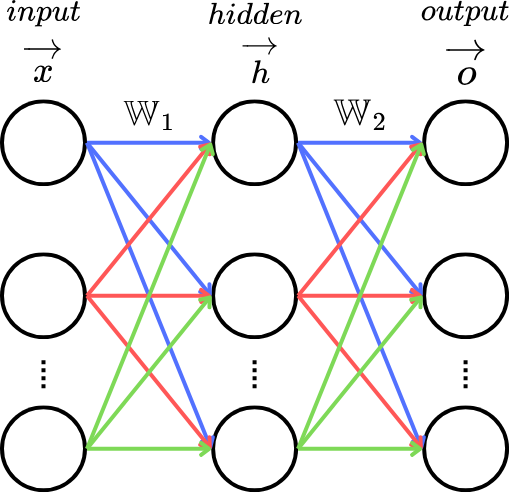
\includegraphics[scale = 0.5]{images/annstructure.png}
    \caption{Structure of the ANN that was developed.}
    \label{fig:annstructure}
\end{figure}

Where a vector of inputs $\overrightarrow{x}$ is fed into the first layer of the network, and this vector is then multiplied by the matrix of weights for the connections between the input layer and the hidden layer, $\mathbb W_1$. There is also a bias that gets added to this weighted summation, denoted by $\overrightarrow{b_1}$. This process results in what is known as the net, which is the weighted summation that is fed into the activation function of the first hidden layer. This is given by Equation \ref{eq:net1} below:

\begin{equation}
    \label{eq:net1}
    \overrightarrow{net_{1}} = \mathbb W_{1} \times \overrightarrow{x} + \overrightarrow{b_1}
\end{equation}

Following the determination of $\overrightarrow{net_{1}}$, this value is then fed into the hidden layer and the activation function is applied, which is given below by Equation \ref{eq:h1}:

\begin{equation}
    \label{eq:h1}
    \overrightarrow{h} = \sigma(\overrightarrow{net_{1}})
\end{equation}

Equation \ref{eq:h1} yields the output from the hidden layer, which is then multiplied by the weights between the hidden and output layer and added to another bias vector to get another net, shown below as:

\begin{equation}
    \label{eq:net2}
    \overrightarrow{net_{2}} = \mathbb W_{2} \times \overrightarrow{h} + \overrightarrow{b_2}
\end{equation}

Finally, the output of the network is computed by applying the activation function to $\overrightarrow{net_{2}}$, as given by:

\begin{equation}
    \label{eq:o1}
    \overrightarrow{o} = \sigma(\overrightarrow{net_{2}}) 
\end{equation}

Neural networks learn by continually updating their weights through a process known as backpropagation, which involves taking the gradient of the difference between your target value and output value, with respect to each individual weight matrix $\mathbb W_{i}$. To update the weights, we want to learn $\mathbb W$'s that minimize the square error function, given by:

\begin{equation}
    \label{eq:squarederrorfunction}
    E[\mathbb W] = \frac{1}{2} \sum_{d \in D}(t_d - o_d)^2
\end{equation}

Where $d$ represents an example from the dataset $D$, $t_d$ is the target label for that example, and $o_d$ is the output of the network. By calculating the gradient of this error function, we get:

\begin{equation}
    \label{eq:sqegradient}
    \nabla{E[\mathbb W]} = \left[ \frac{\partial{E}}{\partial{\mathbb W_o}}, \frac{\partial{E}}{\partial{\mathbb W_1}}, \ldots, \frac{\partial{E}}{\partial{\mathbb W_n}} \right]
\end{equation}

To train the network, we must update the weights according to the following equation:

\begin{equation}
    \label{eq:trainW}
    \mathbb W_i = \mathbb W_i + \Delta{\mathbb W_i}
\end{equation}

Where the incremental change in weight, $\Delta{\mathbb W_i}$, is given by the following equation:

\begin{equation}
    \label{eq:deltaW}
    \Delta{\mathbb W_i} = -\eta \frac{\partial{E}}{\partial{\mathbb W_i}}
\end{equation}

Where $\eta$ is the \textit{learning rate}, which determines the size of the step to be taken during the gradient descent algorithm. The value of $\frac{\partial{E}}{\partial{\mathbb W_i}}$ is given by the following derivation:

\begin{gather}
    \begin{aligned}
        \frac{\partial{E}}{\partial{\mathbb W_i}} &= \frac{\partial}{\partial{\mathbb W_i}} \frac{1}{2} \sum_{d \in D}(t_d - o_d)^2 \\
        &= \frac{1}{2}\sum_{d \in D}\frac{\partial}{\partial{\mathbb W_i}}(t_d - o_d)^2 \\
        &= \sum_{d \in D}(t_d - o_d)\frac{\partial}{\partial{\mathbb W_i}}(t_d - o_d) \\
        &= \sum_{d \in D}(t_d - o_d)\left[-\frac{\partial{o_d}}{\partial{\mathbb W_i}}\right] \\
        &= -\sum_{d \in D}(t_d - o_d)\left[\frac{\partial{o_d}}{\partial{\mathbb W_i}}\right] \\
        \therefore \frac{\partial{E}}{\partial{\mathbb W_i}} &= \sum_{d \in D}(o_d - t_d)\left[\frac{\partial{o_d}}{\partial{\mathbb W_i}}\right]
    \end{aligned}
\end{gather}

Where the value of $\sum_{d \in D}(o_d - t_d)$ is equal to the gradient of the error with respect to the output value $o_d$, as evidenced by Equation \ref{eq:delEdelod}:

\begin{gather}
    \begin{aligned}
        \label{eq:delEdelod}
        \frac{\partial{E}}{\partial{o_d}} &= \sum_{d \in D}(o_d - t_d) \\
        \frac{\partial}{\partial{o_d}}\frac{1}{2}\sum_{d \in D}(t_d - o_d)^2 &= \sum_{d \in D}(o_d - t_d) \\
        \sum_{d \in D}(t_d - o_d)(-1) &= \sum_{d \in D}(o_d - t_d)\\
        \therefore \sum_{d \in D}(o_d - t_d) &= \sum_{d \in D}(o_d - t_d)
    \end{aligned}
\end{gather}

From this, it can be gathered that to update any $\mathbb W_i$, we can use the following equation:

\begin{equation}
    \label{eq:keyweightupdating}
    \mathbb W_i = \mathbb W_i - \eta \left[ \frac{\partial{E}}{\partial{o_d}}\times\frac{\partial{o_d}}{\partial{\mathbb W_i}} \right]
\end{equation}

Meaning that for each layer, the value of $\frac{\partial{o_d}}{\partial{\mathbb W_i}}$ needs to be determined such that each weight matrix can be updated. For the second weight matrix, this derivation is given by Equation \ref{eq:w2update}. The $d$ subscript is dropped as it was assumed that stochastic gradient descent would be employed, which obviously is performed on each training example $d \in D$.

\begin{gather}
    \begin{aligned}
        \label{eq:w2update}
        \frac{\partial{o}}{\partial{\mathbb W_2}} &= \frac{\partial}{\partial{\mathbb W_2}}\sigma(\overrightarrow{net_2}) \\
        &= \frac{\partial}{\partial{\mathbb W_2}}\sigma(\mathbb W_2 \sigma(\mathbb W_1 \overrightarrow{x})) \\
        \therefore \frac{\partial{o}}{\partial{\mathbb W_2}} &= \sigma'(\overrightarrow{net_2})h
    \end{aligned}
\end{gather}

Similarly, this process was repeated for $\mathbb W_1$:

\begin{gather}
    \begin{aligned}
        \label{eq:w1update}
        \frac{\partial{o}}{\partial{\mathbb W_1}} &= \frac{\partial}{\partial{\mathbb W_1}}\sigma(\overrightarrow{net_2}) \\
        &= \frac{\partial}{\partial{\mathbb W_1}}\sigma(\mathbb W_2 \sigma(\mathbb W_1 \overrightarrow{x})) \\
        &= \sigma'(\overrightarrow{net_2})\frac{d}{d{\mathbb W_1}}\left[ \mathbb W_2 \sigma(\mathbb W_1 \overrightarrow{x}) \right]\\
        \therefore \frac{\partial{o}}{\partial{\mathbb W_1}} &= \sigma'(\overrightarrow{net_2})\mathbb W_2 \sigma'(\overrightarrow{net_1})\overrightarrow{x}
    \end{aligned}
\end{gather}

The question therefore arose, how will the bias be updated? It was determined that the bias would be updating using a similar approach to Equation \ref{eq:trainW}, where the bias updating equation is given below as:

\begin{equation}
    \label{eq:trainBias}
    b_i = b_i - \eta \frac{\partial{E}}{\partial{b_i}}
\end{equation}

Where the partial derivative of error with respect to the bias value $b_i$ is given by:

\begin{gather}
    \begin{aligned}
        \label{eq:biasderivation}
        \frac{\partial{E}}{\partial{b_i}} &= \frac{\partial}{\partial{b_i}}\left[ \frac{1}{2} \sum_{d \in D}(t_d - o_d)^2 \right] \\
        &= \frac{1}{2}\sum_{d \in D} \frac{\partial}{\partial{b_i}}(t_d - o_d)^2 \\
        &= \sum_{d \in D}\frac{\partial}{\partial{b_i}}(t_d - o_d) \\
        &= \sum_{d \in D}(t_d - o_d)\frac{\partial}{\partial{b_i}}(-o_d) \\
        \therefore \frac{\partial{E}}{\partial{b_i}} &= \sum_{d \in D}(o_d - t_d)\frac{\partial{o_d}}{\partial{b_i}}
    \end{aligned}
\end{gather}

Where the value of $\sum_{d \in D}$ is known by Equation \ref{eq:delEdelod}, which implies that the partial derivative of error with respect to bias is equal to:

\begin{equation}
    \label{eq:delEdelbias}
    \frac{\partial{E}}{\partial{b_i}} = \frac{\partial{E}}{\partial{o_d}} \times \frac{\partial{o_d}}{\partial{b_i}}
\end{equation}

The expanded equation of the output from our network, with biases included, is given below within Equation \ref{eq:outputwithbias}. The biases were initially neglected when determining the weight matrices as they are not functions of the weight, and therefore were dropped when the partial derivative of error with respect to the weight matrices was performed. 

\begin{equation}
    \label{eq:outputwithbias}
    \overrightarrow{o} = \sigma(\mathbb W_2 \sigma(\mathbb W_1 \overrightarrow{x} + \overrightarrow{b_1}) + \overrightarrow{b_2})
\end{equation}

Therefore, we just need to determine the value of $\frac{\partial{o_d}}{\partial{b_i}}$ for each layer. For $b_2$, this is done as follows:

\begin{gather}
    \begin{aligned}
        \frac{\partial{o_d}}{\partial{b_2}} &= \frac{\partial}{\partial{b_2}}\sigma(\overrightarrow{net_2} + \overrightarrow{b_2}) \\
        \frac{\partial{o_d}}{\partial{b_2}} &=\sigma'(\overrightarrow{net_2})
    \end{aligned}
\end{gather}

For $b_1$, this is done as follows:

\begin{gather}
    \begin{aligned}
        \frac{\partial{o_d}}{\partial{b_1}} &= \frac{\partial}{\partial{b_1}} \sigma(\mathbb W_2 \sigma(\mathbb W_1 \overrightarrow{x} + \overrightarrow{b_1}) + \overrightarrow{b_2})\\
        \frac{\partial{o_d}}{\partial{b_1}} &= \sigma'(\overrightarrow{net_2})\mathbb W_2 \sigma'(\overrightarrow{net_1})
    \end{aligned}
\end{gather}

The general workflow for utilizing the neural network is as follows:

\begin{enumerate}
    \item A neural network object is instantiated from a class, specifying the input size, the hidden layer size, and output size.
    \item This network is then trained, using a training function that is contained within the object. This training procedure calculates a forward pass first by passing the input vector through the network, which yields an output. This output, as well as the target values from the input vector and a learning rate are passed through a backward pass, which updates the weights using the backpropagation equations determined above.
    \item Once the network has been trained, it can be tested by passing it features and labels, where it calculates the accuracy of the model based on how many it correctly classifies.
\end{enumerate}

With all of the pertinent equations for the backpropagation algorithm determined, as well as the workflow, the focus then turned towards the actual implementation of the neural network through code for performing classification on the given dataset.

\subsection{Implementation Details}

This section outlines all details related to the implementation of the neural network, including the development platform and libraries used, the programmatic structure, the data structures used, the choice of hyperparameters, the details about the dataset, the pre-processing performed, as well as the design of the implementation. Experimental results are also examined. 

\subsubsection{Development Platform \& Libraries Used}

As was previously mentioned, all code written to implement the neural network with backpropagation was written in Python 3. The code was written on a Windows operating system, and was not tested on other operating systems, but it is assumed that it will run on any system that can run the Python programming language. The development of this algorithm was done using Microsoft's Visual Studio Code. The environment was configured to run Jupyter Notebook .ipynb files, which due to their ability to run code one cell at a time, are favoured for machine learning development. The Python 3 kernel that was utilized within this .ipynb environment was Python 3.12.5. Code versioning was controlled through Git utilizing a remote repository hosted on GitHub. The neural network itself, as well as the backpropagation algorithm, were written completely from scratch using Python's built-in functionalities as well as the \textit{Numpy} Python library for mathematical operations. The \textit{Pandas} Python library was utilized for data manipulation and exploratory analysis, and the \textit{scikit-learn} machine learning Python library was used to apply pre-processing to the data, as well as performing the train/test split. It must be noted that this machine learning library was not used for anything other than splitting data and applying standardization. It was not incorporated within the actual neural network class, and did not contribute to the development of the neural network other than being a tool for data separation and scaling. Finally, the \textit{matplotlib} and \textit{seaborn} Python libraries were utilized for visualization of both training and testing results. 

\subsubsection{Program Structure}

% talk about object oriented approach, maybe given example of the class, workflow of the document starting from loading data to testing.
\subsubsection{Data Structures Used}
% talk about pandas and numpy data structures used and how they were utilized.

\subsubsection{Hyperparameter Selection}\label{ANNhyperparameterselection}

% only real hyperparameters used were the epochs, learning rate, and the number of hidden neurons in the first layer. talk about them.

% justify why only 1 hidden layer was chosen

\subsection{Dataset Details}

\subsection{Data Pre-processing}

\subsection{Experimental Results}

\section{Conclusion}

\newpage

% Bibliography/Reference Stuff
\bibliographystyle{abbrv}
\bibliography{main}
\end{document}